\documentclass[a4paper,12pt]{article} 

%%% Работа с русским языком
\usepackage{cmap}					% поиск в PDF
\usepackage{mathtext} 				% русские буквы в фомулах
\usepackage[T2A]{fontenc}			% кодировка
\usepackage[utf8]{inputenc}			% кодировка исходного текста
\usepackage[english,russian]{babel}	% локализация и переносы

%%% Дополнительная работа с математикой
\usepackage{amsmath,amsfonts,amssymb,amsthm,mathtools, gensymb} % AMS
\usepackage{icomma} % "Умная" запятая: $0,2$ --- число, $0, 2$ --- перечисление

%%Таблица
\usepackage[table,xcdraw]{xcolor}
\usepackage{caption}
\usepackage{subcaption}
\usepackage{floatrow}
\floatsetup[table]{capposition=top}
\floatsetup[wrapfigure]{capposition=bottom}


%% Номера формул
\mathtoolsset{showonlyrefs=true} % Показывать номера только у тех формул, на которые есть \eqref{} в тексте.

%% Шрифты
\usepackage{euscript}	 % Шрифт Евклид
\usepackage{mathrsfs} % Красивый матшрифт

%% Свои команды
\DeclareMathOperator{\sgn}{\mathop{sgn}}

%% Перенос знаков в формулах (по Львовскому)
\newcommand*{\hm}[1]{#1\nobreak\discretionary{}
{\hbox{$\mathsurround=0pt #1$}}{}}

%% Стиль страницы
\usepackage{fancyhdr}

%% Для рисунков
\usepackage{graphicx}
\usepackage[export]{adjustbox}
\usepackage{float}
\usepackage{ragged2e}
\usepackage{wrapfig}

%Отступы и поля 
\textwidth=20cm
\oddsidemargin=-2cm
\topmargin=-2cm
\textheight=25cm

\pagestyle{fancy}
\begin{document}
\begin{titlepage}
\begin{center}
%\vspace*{1cm}
\large{\small ФЕДЕРАЛЬНОЕ ГОСУДАРСТВЕННОЕ АВТОНОМНОЕ ОБРАЗОВАТЕЛЬНОЕ\\ УЧРЕЖДЕНИЕ ВЫСШЕГО ОБРАЗОВАНИЯ \\ МОСКОВСКИЙ ФИЗИКО-ТЕХНИЧЕСКИЙ ИНСТИТУТ\\ (НАЦИОНАЛЬНЫЙ ИССЛЕДОВАТЕЛЬСКИЙ УНИВЕРСИТЕТ)\\ ФАКУЛЬТЕТ АЭРОКОСМИЧЕСКИХ ТЕХНОЛОГИЙ}
\vfill
\line(1,0){430}\\[1mm]
\huge{Лабораторная 3}\\
\huge\textbf{После пузырька можно уже всё}\\
\line(1,0){430}\\[1mm]
\vfill
\begin{flushright}
\normalsize{Рогозин Владимир}\\
\normalsize{\textbf{Группа Б03-106}}\\
\end{flushright}
\end{center}
\end{titlepage}
\fancyhead[L] {Лабораторная 3}

\textbf{Пункт 1:}
a) Уже из самого первого примера на С с простейшей функуцией без аргументов и возвращаемых значений видно, что в 32-х битной версии много дополнительных действий, а именно пуши регистров и действия с ними.   
\begin{figure}[H]\label{fig: BezArgumentovFuncNaC 64 and 32}
    \subfloat[на C 32-х битная система]{
    \begin{minipage}[t]{0.4\textwidth}
        \centering
        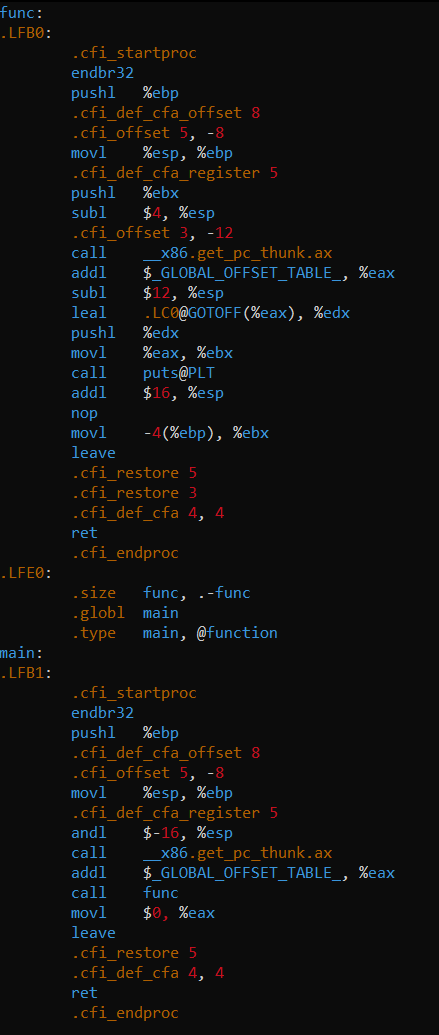
\includegraphics[width = 0.85\textwidth]{1aC32.png}
    \end{minipage}}
    \subfloat[на C 64-х битная система]{
    \begin{minipage}[t]{0.4\textwidth}
        \centering
        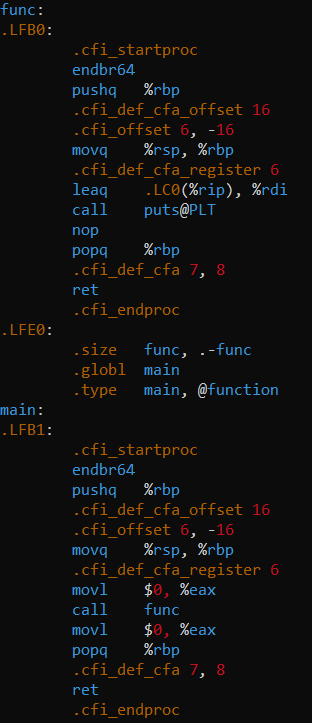
\includegraphics[width = 0.865\textwidth]{1aC64.png}
    \end{minipage}}
\end{figure}

\begin{figure}[H]\label{fig: 1aProgramme C and C++}
    \subfloat[Код программы на С]{
    \begin{minipage}[t]{0.4\textwidth}
        \centering
        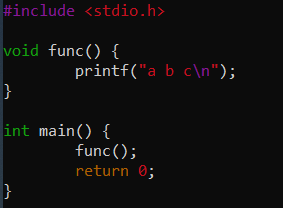
\includegraphics[scale = 0.57]{1aCProgramme.png}
    \end{minipage}}
    \subfloat[Код программы на С++]{
    \begin{minipage}[t]{0.4\textwidth}
        \centering
        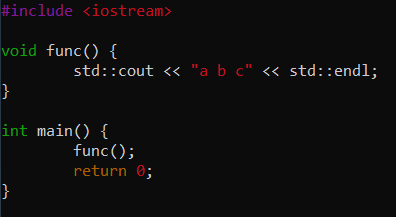
\includegraphics[scale = 0.53]{1aCppProgramme.png}
    \end{minipage}}
\end{figure}

\begin{figure}[H]\label{fig: 1aCpp64}
    \centering
    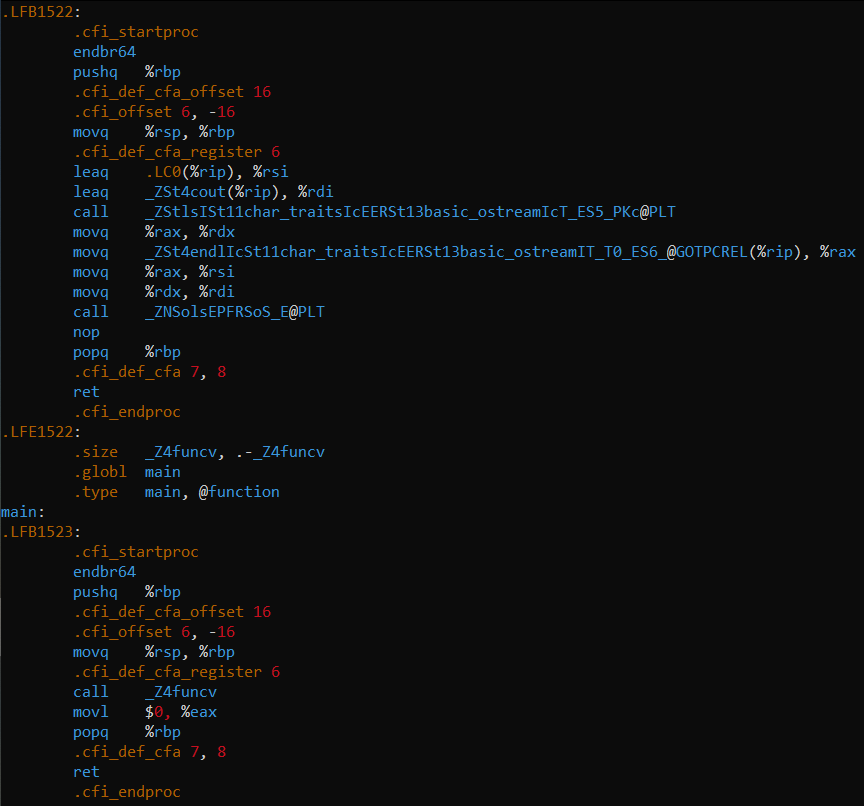
\includegraphics[scale = 0.4]{1aCpp64.png}
    \caption{Листинг программы на С++ 64-х битной системы}
\end{figure}

На C++ ситуация примерно такая же, в 32-х битной версии присутствуют какие-то дополнительные пуши регистров, в 64-х битной версии такого почти нету, за исключением пушей, связанных, как  мне кажется, с $std::cout$ и $std::endl$. 

b) Для функции без аргумеетов, но с возвращаемым значением типа $int$ дела обстоят практически одинаково что для С++, что для С, независимо от разрядности системы. Везде под возвращаемый $int$ выделяется 16 байт (почему-то), только в С++ немного хуже дела обстоят с названиями (с человеческой точки зрения).

c) Далее, функция, возвращающая $int$, с одним аргументом того же типа. Здесь видны различия между 64-х и 32-х битными системами. В 32-х битной аргумент, который потом передаётся в функцию, перед вызовом функции кладётся в стек, и потом лежит в стеке перед функцией, причём если внутри функции есть арифметические операции с аргументом, то они производятся со значением, лежащим в стеке перед функцией. В 64-х битной системе аргумент запоминается в отдельный регистр (у меня был $edi$), после вызова функции значение с этого регистра копируется в стек, и операции проводятся со значением, лежащим в стеке после функции. Разницы между С и С++ опять же почти нету. Под результат функции (одно число $int$) и там и там выделяется 16 байт.

d) Теперь функция, которая возвращает $int$ и принимает два аргумента типа $int$. Всё почти так же как и в предыдущем случае. В 32-х битном варианте резервируется под возвращаемое значение место в стеке (опять 16 байтов на один $int$), затем в стек пушатся аргументы функции, затем функция, потом производятся все арифметические операции, значения для которых передаются в регистры из стека (оттуда куда до этого пушились аргументы), после завершения работы функции на вершине стека остаётся возвращаемое значение. В 64-х битной системе, как и в предыдущем случае, используются дополнительные регистры (теперь $edi$ и $esi$) для хранения значений аргументов. Значения их этих регистров копируются в стек функции, там же и проделываются операции с числами. Результат работы программы после её завершения также остаётся на вершине стека, на один $int$ выделяется 16 байт. Различия между С и С++ всё также только в названиях переменных.     

\textbf{Пункт 2:}
a) Разберёмся с локальными переменными. Сначала посмотрим листинг с одной локальной переменной.
\begin{figure}[H]\label{fig: 2aCpp32}
    \centering
    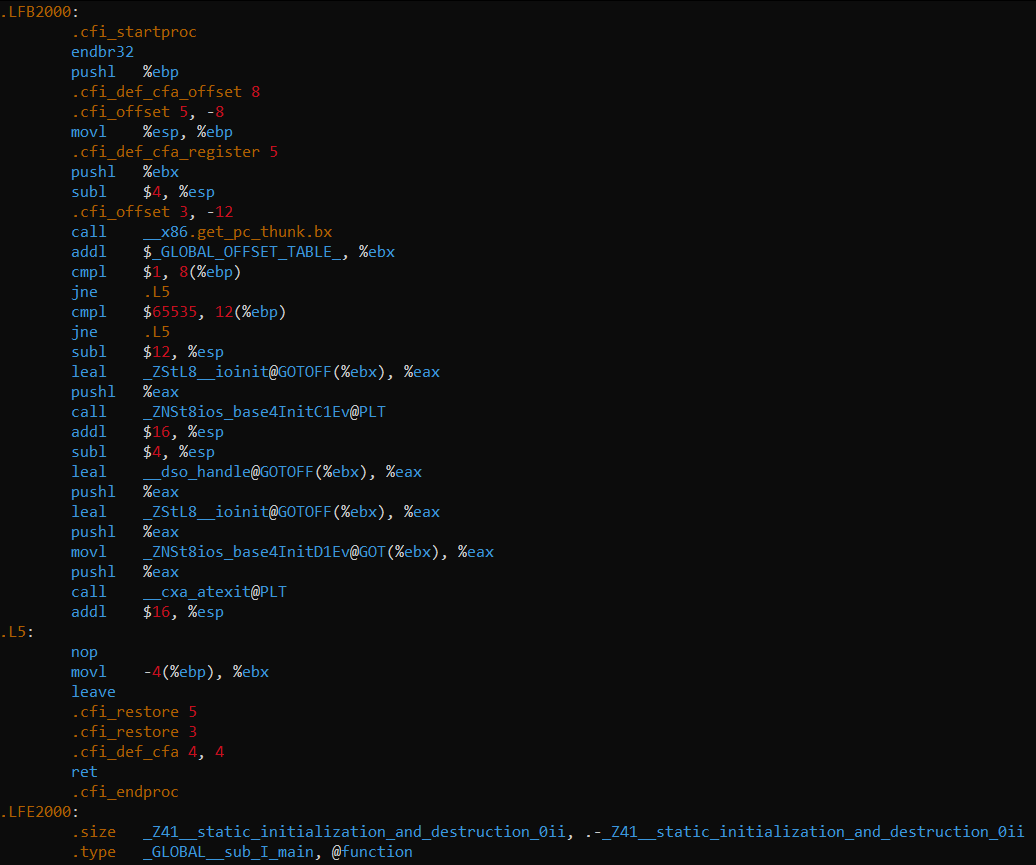
\includegraphics[width = 0.8 \textwidth]{2aCpp32.png}
    \caption{Функции после $main$, 32-х битная система}
\end{figure}
В языке С все достаточно предсказуемо, локальная переменная кладётся на вершину стека $main$'а, различия между 32-х и 64-х разрядной системой почти нету. Однако дело обстоит совсем по-другому с С++. В функции $main$ все без изменений по сравнению с С, но после $main$'а что в 32-х битной, что в 64-х битной появляются ещё дополнительные функции, судя по некоторым различимым словам, это похоже на конструктор и деструктор класса $int$.

b) Теперь на очереди программа с парой локальных переменных типа $int$. В С, как в 32-х так и в 64-х битной системе, обе переменные просто кладутся на вершину стека $main$'а. В $main$'е листинга С++ всё идентично листингу на С, но после него опять 
идут дополнительные функции, которые абсолютно такие же, что и в случае одной локальной переменной, они на скринах листинга ниже и выше этого текста.

\begin{figure}[H]\label{fig: 2aCpp64}
    \centering
    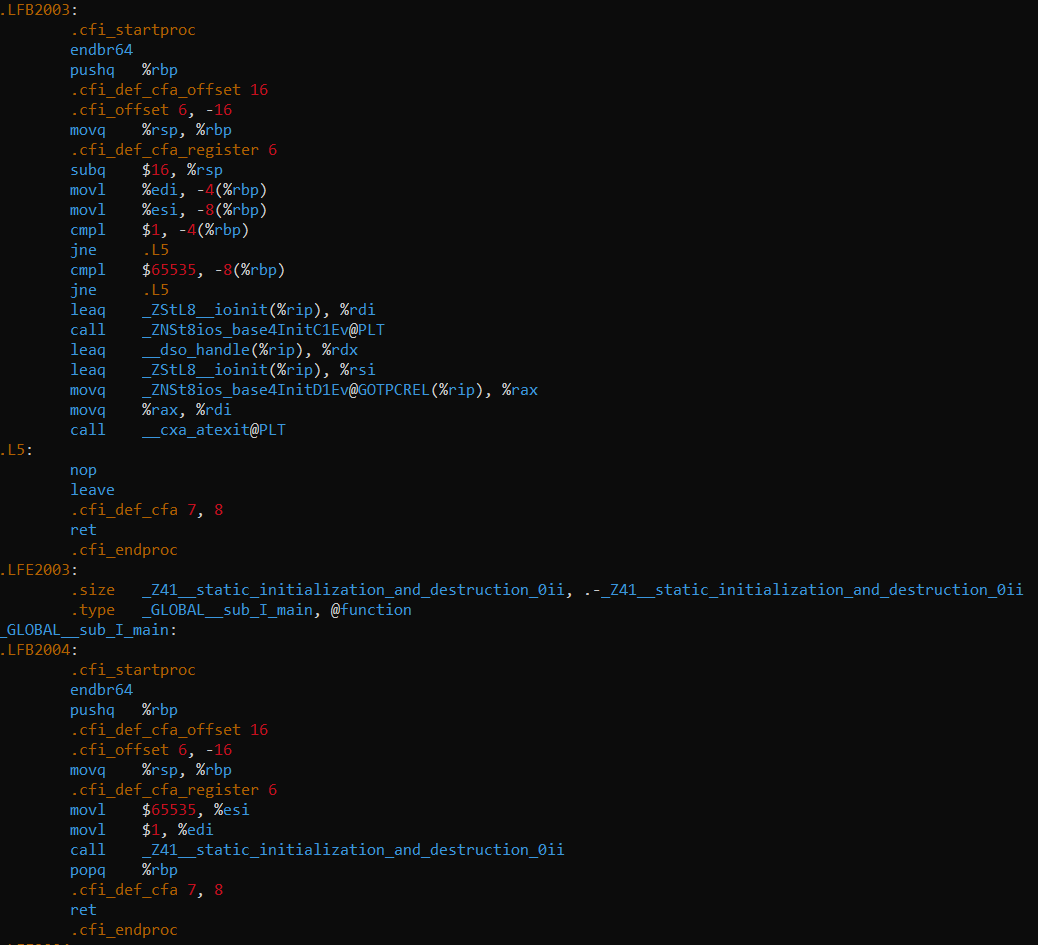
\includegraphics[width = 0.8 \textwidth]{2aCpp64.png}
    \caption{Функции после $main$, 64-х битная система}
\end{figure}

c) При создании статического массива из $int$'ов на С++ после $main$'а присутствуют те же самые дополнительные функции (похоже конструктор деструктор), которых нету на С, однако основной интерес представляют изменения в $main$'е. И в С, и в С++, и в 32-х битной, и в 64-х в стеке выделяется место под элементы массива (опять больше  чем надо), но перед этим выполняется команда $movq$ с первым операндом $\% fs:40$. Вся эта цепочка действий нужна для того, чтобы в конце работы функции проверить стек на переполненность, в регистре по адресу $fs:40$ лежит определенная константа, значения которой сравниваются в начале и в конце программы, если что-то идёт не как должно, то вызывается функция stack chk fail. В 32-х битной системе используется адрес $gs:20$.           

\begin{figure}[H]\label{fig: 2вC64 and 2вC++64}
    \subfloat[Статический массив на С]{
    \begin{minipage}[t]{0.4\textwidth}
        \centering
        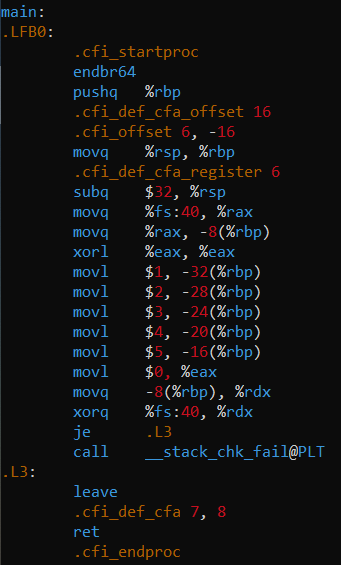
\includegraphics[scale = 0.6]{2вC64.png}
    \end{minipage}}
    \subfloat[Статический массив на С++]{
    \begin{minipage}[t]{0.4\textwidth}
        \centering
        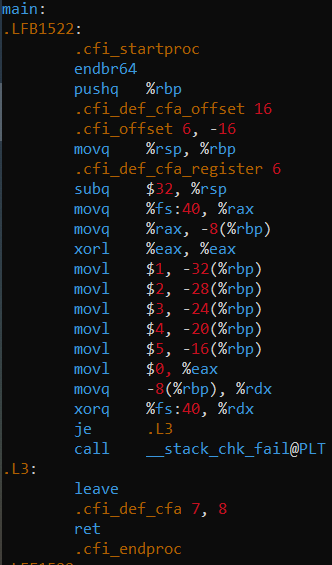
\includegraphics[scale = 0.6]{2вCpp64.png}
    \end{minipage}}
\end{figure}

d) Далее, динамический массив. Разницы между С и С++ опять почти нету, но большие отличия в листингах для различных систем.  В 32-х битной перед и после пуша регистров, указывающих на вершину и дно стека ($esp$ и $ebp$ соответственно) кладутся в стек ещё и $ebx$ и $ecx$, причем до этого в $main$'е регистр $ebx$ вообще никак не используется, то есть по сути там лежит ненужный мусор. В каждой из систем в стеке хранится адрес на первый элемент выделенной памяти по которому и можно обращаться к любому элементу дин. массива. В 32-х битной системе количество выделенных байт (число) пушится в стек перед вызовом $new$($malloc$), в 64-х -- хранится в отдельном регистре (здесь это $edi$).   
\begin{figure}[H]\label{fig: 2гCpp32 and 2гCpp64}
    \subfloat[Динамический массив на С++, 32 бита]{
    \begin{minipage}[t]{0.4\textwidth}
        \centering
        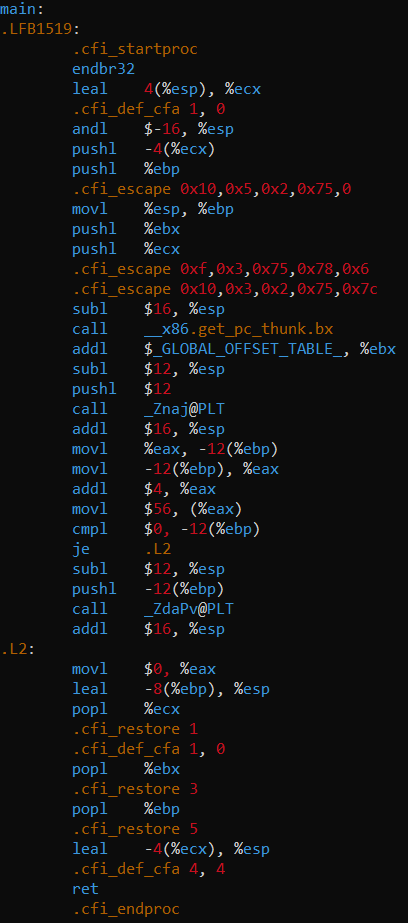
\includegraphics[scale = 0.45]{2гCpp32.png}
    \end{minipage}}
    \subfloat[Динамический массив на С++, 64 бита]{
    \begin{minipage}[t]{0.4\textwidth}
        \centering
        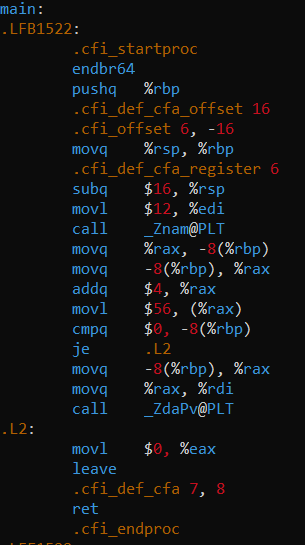
\includegraphics[scale = 0.75]{2гCpp64.png}
    \end{minipage}}
\end{figure}

\textbf{Пункт 3:} 
a) Двигаемся к структурам, сначала, не создавая экземпляра, просто объявим структуру с четырьмя различными полями $int$, $char$, $float$ и $short$. В обоих языках в листинге просто по сути пустой $main$(что и логично), видимо пока нету экземпляра класса это никак не отражается на листинге. В С++ $main$ также пуст, но функции после него (которые я считал конструктором и деструктором класса $int$) остались абсолютно такими же, вероятно это все же что-то другое, продолжим это выяснять дальше.

b) Теперь создадим глобальную переменную структуры и попробуем изменить пару её полей в $main$'е. Обращение происходит как и в случае c глобальным массивом, причем выделяется под каждое поле 4 байта, хотя некторые из них весят меньше . Перед $main$'ом объявляется глобальная переменная переменная. Принципиальных различий между С и С++ все также нет.
\begin{figure}[H]\label{fig: 3бCpp32 and 3бCpp64}
    \subfloat[Глобальная структура на С++, 32 бита]{
    \begin{minipage}[t]{0.4\textwidth}
        \centering
        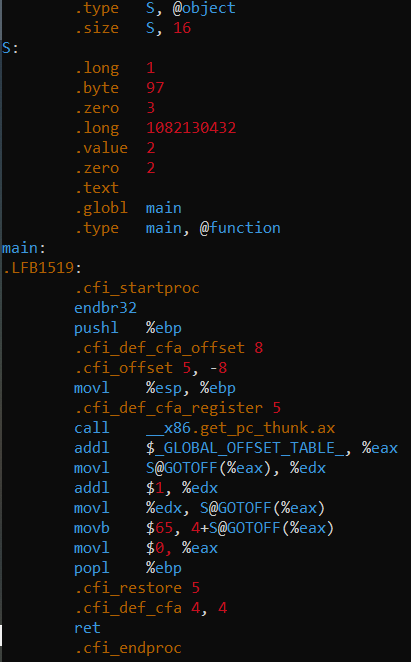
\includegraphics[scale = 0.55]{3бCpp32.png}
    \end{minipage}}
    \subfloat[Глобальная структура на С++, 64 бита]{
    \begin{minipage}[t]{0.4\textwidth}
        \centering
        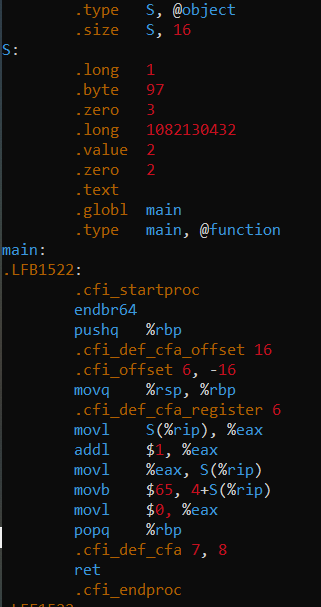
\includegraphics[scale = 0.6]{3бCpp64.png}
    \end{minipage}}
\end{figure}

c) Теперь в ту же структуры добавим статический массив. Ничего сверхъестественного не получаем, статический массив размера $N$ по сути эквивалентен $N$ переменным одного типа, так его и представляет компилятор, как бы развертывает массив в $N$ новых полей одного типа. Принципиальных различий в разных системах и языках нету.

d) Тут передадим структуру в функцию (пока что не по указателю или ссылке). В обеих системах и обоих языках перед функцией в стек пушатся копии всех полей структуры (элементы массива пушатся поочереди) таким образом, что наверху оказывается первое по счёту поле. Различие в том, что в 32-х битной системе это делается с помощью команды $pushl$, а в 64-х битной это делается командой $movq$, используя адрес ячейки в стеке, к тому же, даже если переменные весят меньше 8 байт, к примеру две по 4 байта, их слепляют в одну восьмибайтовую, достать одно из двух значений конечно можно дописав к команде $mov$ окончание $l$ и указав правильный адрес.

e) Если сделать возвращаемым значением сделать структуру, то в этом случае также, как и когда функция возвращала целое число, в стеке перед вызовом функции резервируется место под возвращаемое значение, затем в стек пушатся все аргументы, потом вызывается функция. после завершения работы на вершине стека оказывается возвращаемая структура. Различие между системами только в способе заполнения стека, в 32-х битной с помощью команды $pushl$, в 64-х -- $movq$.  

f) В этом пункте взглянем на методы класса в С++. При создании экземпляра класса  вызывается его конструктор, если у класса есть поля, под их значения выделяется место в стеке перед вызовом самой функции (конструктора). После этого вызывается функция, куда передаются адреса для записи значений полей, куда в итоге и попадают значения полей экземпляра класса. Если вызывается метод класса, то, если он использует поля класса, в функцию передаются как бы неявные аргументы -- поля, метод работает как обчная функция, если он меняет поля, то по сути это принимающая на вход указатель и меняющая по нему значение функция (что опять же логично очень даже). 

g) Операторы. Операторы это те же функции. Работают также, результат операции отправляется в заранее заготовленную ячейку памяти. Единственное, в 32-х битной системе результат записывается в нужную ячейку в конце выполнения функции, в 64-х битной результат возвращается в регистре, после чего записывается из регистра в нужную часть памяти.  

\textbf{Пункт 4:}
а) Структуру в функцию мы уже передавали в пункте 3d), поэтому тут все тоже самое.

b) Теперь передадим структуру по указателю. Здесь все также достаточно ожидаемо, просто теперь функция использует не скопированные значения полей, а адреса ячеек, в которых лежат эти значения. Обращаясь по этим адреса, функция меняет сам объект, а не его копию. Отличие между 32-х и 64-х битной системами в том, что в 64-х битной когда полей мало, то их адреса передаются в функцию через регистры(адрес записывается в регистр, потом переписывается из регистра в стек функции после её вызова), а в 32-х битной всегда адреса пушатся в стек перед вызовом функции.    

c) Ссылки на очереди. Передача в функцию по ссылке в ассемблерном листинге никоим образом не отличается от передачи по указателю. Все абсолютно также, как и в предыдущем пункте.

d) В этом пункте рассмотрим передачу в функцию с помощью rvalue-ссылок. В этом случае просто результат промежуточного действия записывается в одну из ячееку стека, адрес которой потом передаётся в функцию.  
 
\textbf{Пункт 5:} 
a) Создадим структуру со статическим массивом в 100000 элементов значением 0, передадим её аргументом в функцию. Листинги программы приведены ниже: 
\begin{figure}[H]\label{fig: 5aCpp32 and 5aCpp64}
    \subfloat[Жирная структура в аргументе С++, \\ 32 бита]{
    \begin{minipage}[t]{0.4\textwidth}
        \centering
        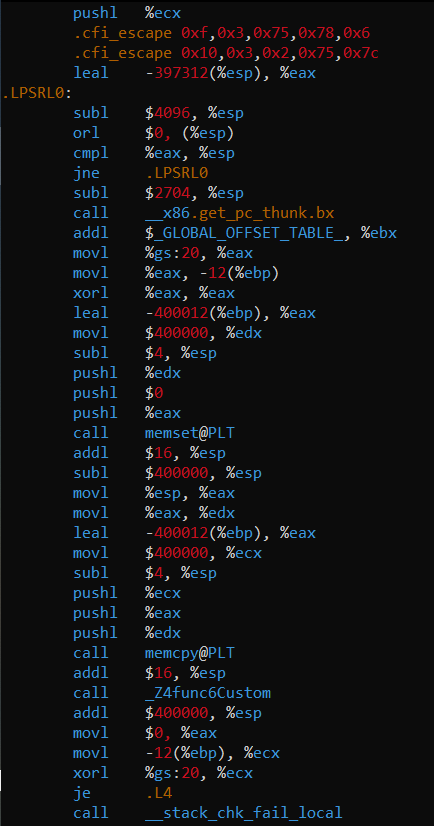
\includegraphics[scale = 0.42]{5aCpp32.png}
    \end{minipage}}
    \subfloat[Жирная структура в аргументе С++, \\ 64 бита]{
    \begin{minipage}[t]{0.4\textwidth}
        \centering
        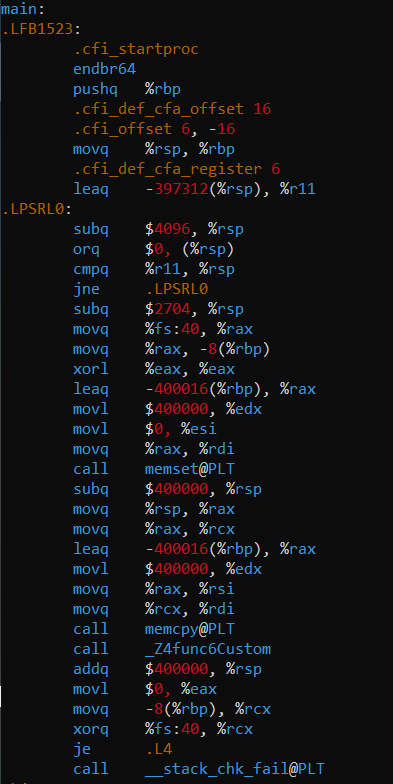
\includegraphics[scale = 0.44]{5aCpp64.png}
    \end{minipage}}
\end{figure}
Как видно, сначала при создании экземпляра структуры выделяется 400000 байт, значения задаются с помощью функции memset, которая принимает на вход адрес первого элемента массива, значение, которое нужно присвоить элементам массива(здесь это 0), и длину массива. Различие между системами в том, что в 32-х битной эти аргументы функции memset пушатся в стек, а затем функция уже берет их оттуда, а в 64-х битной системе аргументы кладутся в регистры, откуда потом функция их использует. Но это относится к созданию экземпляра класса, что касается его передачи в функцию (точнее его копии), то тут дело обстоит примерно также, за исключением того, что для копирования массива при передачи в функцию используется функция memcpy. Она принимает на вход адрес куда копировать, адрес откуда копировать и количество элементов. Аргументы передаются в функцию таким же образом, по-разному в разных системах. Также заметим, что первое выделение места под структуру происходит не единовременным вычитанием 400000 байт из $rsp$($esp$), а в цикле, вычитая по 4096 байт (вот это выглядит странным, плюс тот факт, что с числом, лежащим в ячейке на которую указывает промежуточное значение $rsp$($esp$), прозводится логическое или, где второй операнд есть 0). 

b) Теперь огромную структуру будем возвращать из функции, принимающей на вход тоже большую структуру. По сути, ничего принципиально отличающегося от предыдущего случая тут нету, просто больше копирований туда-сюда. Заранее выделяется место в стеке под возвращаемое значение (причем оно оказалось ниже в стеке, чем значение полей изначально созданной структуры, копия которой потом передаётся в функцию), с помощью memcpy сначала копируется на вершину весь массив как аргумент функции, затем, после операций, используя тот же memcpy, измененные значения копируются на дно стека, после этого работа функции заканчивается.

c) Если создать большую структуру внутри функции, то с помощью команды memset в стеке функции будет создан экземпляр структуры точно также, как и в стеке $main$'a.

d) При изменении размера структуры вроде как в обеих системах ничего, кроме размера выделяемой памяти, не меняется.

\textbf{Пункт 6:}
Напишем рекурсивную функцию и посмотрим на её листинг. Просто из функции вызывается эта же функция.  
\begin{figure}[H]\label{fig: 6C32 and 6Cpp64}
    \subfloat[Рекурсия на С, 32 бита]{
    \begin{minipage}[t]{0.4\textwidth}
        \centering
        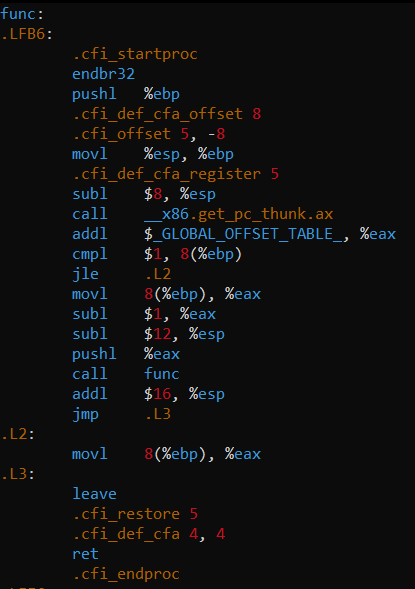
\includegraphics[scale = 0.5]{6С32.png}
    \end{minipage}}
    \subfloat[Рекурсия на С++, 64 бита]{
    \begin{minipage}[t]{0.4\textwidth}
        \centering
        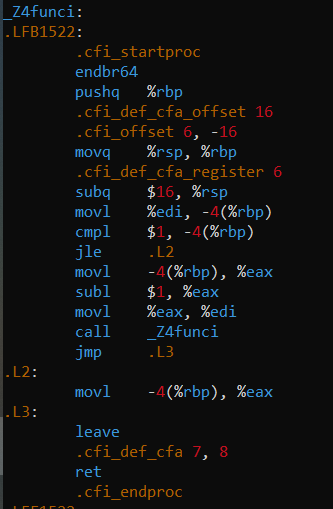
\includegraphics[scale = 0.57]{6Cpp64.png}
    \end{minipage}}
\end{figure}

\end{document}
